\chapter{The Graph Neural Network Model}


\section{Graph Neural Network}

The Graph Neural Network (GNN) is a flexible neural network architecture that is based on two local operators on a graph $G = (V, E)$. Given some input signal $F \in \mathbb{R}^{n \times p}$ on the vertices of an n-vertex graph, we consider two operators that act locally on this signal as well as a non-linearity operator.\\

\begin{definition}Define the \textit{degree operator} as a map $D : F \mapsto D(F)$ where $$(D(F))_i := deg(i) \cdot F_i.$$  And $deg(i)$ is the degree of vertex $i \in V$.  
\end{definition}
\begin{definition}Define the \textit{adjacency operator} as a map $W: F \mapsto W(F)$ where $$(W(F))_i:= \sum_{j\sim i }F_j.$$ And $i \sim j$ means vertex $i$ is adjacent to vertex $j$. 
\end{definition}

\begin{definition}Define the \textit{pointwise nonlinearity operator} as a map $\eta_{\theta}: \mathbb{R}^p \cdot \mathbb{R}^p \rightarrow \mathbb{R}^q$ parametrized by some $\theta \in \mathbb{R}^l$ trainable. An example of such an operator is the convolution operator used in convolutional neural networks.\\
\end{definition}

\begin{figure}
\begin{center}
  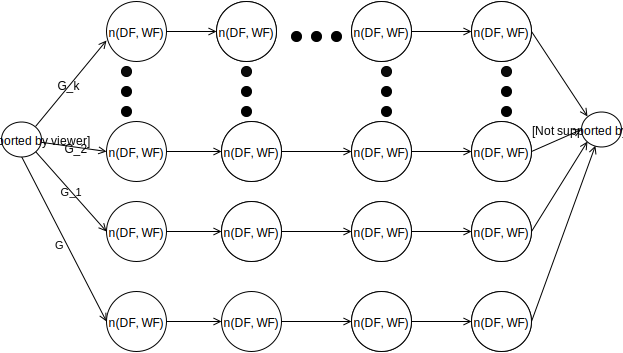
\includegraphics[width=\textwidth]{GNN.png}
  \caption{An example of an architecture constructed from operators D, W and $\theta$}
  \label{fig:GNN}
 \end{center}
\end{figure}

Immediately from this definition, we get that after one layer of applying $D$ and $W$ allows us to recover the graph Laplacian operator.  To be precise, let $F$ be a $p$-dimensional signal on $G$.  Then if we define $$ \eta(DF, WF) := DF - WF$$ we recover the unnormalized graph Laplacian.  If we allow add to the operators above an additional $D^{-1/2}$ and $D^{-1}$ operator (which will be analogous to $D$ defined above, only with entries multiplied by the entires of $D^{-1/2}$ and $D^{-1}$), we will be able to recover the symmetric and random walk Laplacians.  Furthermore, by stacking together several of the Laplacian modules, and allowing ourselves to renormalize the signal after each  module, we are able to recreate the power method.  Therefore the expressive power of this GNN includes approximations to eigendecompositions.\\

\subsection{Related Work}
The GNN was first proposed in \cite{GNN} as a way to approximate functions on graphs. Bruna et al. also generalized convolutions for signals on graphs in \cite{Bruna}.  The idea there is that the convolution neural network architecture so successful for image data, can be construed as decomposing the image signals into the very rapidly decaying Fourier basis.  Rapidly decaying because images lie on such regular graphs (in particular grids). The right generalization is then to use the graph Laplacian's eigenbasis to create a general graph convolution.  The authors successfully applied this neural network for signals on meshes.  Kipf and Welling showed more recently in \cite{kipf2016semi} the GNN with a symmetric Laplacian module, with only two layers, can be quite effective as a embedding mechanism for graph signals.  They applied their network to semi-supervised learning problems where some graph nodes were labelled but others were not.\\

The present work is the first time a neural network has been applied to community detection.  In particular this means the graphs we are dealing with are far larger and far sparser then all previous works.  The GNN architecture family is quite general, so it required taking the most expressive combination of modules to be able to approximate spectral algorithms of interest mentioned in the last chapter.  We are able to show that our version of the GNN can compete with spectral algorithms in doing spectral clustering on the SBM in even the hardest of regimes (detectability).  This will not work with previous GNN architectures mentioned above.  In addition, we are not doing an eigendecomposition, which is required of spectral algorithms.  Thus making the network more efficient computationally.  %Lastly we apply the GNN to extremely large graphs, with millions of nodes.  These real datasets have ground truth communities which we compare the performance of.  



